\documentclass[a4paper,12pt]{article} % тип документа

% report, book

% Рисунки
\usepackage{graphicx}
\usepackage{wrapfig}
\usepackage{mathtext}
\usepackage[left=2cm,right=2cm,
    top=2cm,bottom=2cm,bindingoffset=0cm]{geometry}

\usepackage{hyperref}
\usepackage[rgb]{xcolor}
\hypersetup{				% Гиперссылки
    colorlinks=true,       	% false: ссылки в рамках
	urlcolor=blue          % на URL
}

%  Русский язык
\usepackage[T2A]{fontenc}			% кодировка
\usepackage[utf8]{inputenc}			% кодировка исходного текста
\usepackage[english,russian]{babel}	% локализация и переносы


% Математика
\usepackage{amsmath,amsfonts,amssymb,amsthm,mathtools} 


\usepackage{wasysym}

\author{Анна Назарчук Б02-109}
\title{1.3.3 Измерение вязкости воздуха по течению в тонких трубках}
\date{}
\begin{document}
\maketitle
\section{Аннотация}
В работе измеряется коэффицент вязкости воздуха при помощи воздуха, движущего в тонких трубках с разными скоростями, имея разные числа Рейнольдса.

\textbf{Цель работы:} экспериментально исследовать свойства течения газов по тонким трубкам при различных числах Рейнольдса; выявить область применимости закона Пуазейля и с его помощью определить коэффициент вязкости воздуха.

\textbf{В работе используются:}  система подачи воздуха (компрессор, поводящие трубки); газовый счетчик барабанного типа; спиртовой микроманометр с регулируемым наклоном; набор трубок различного диаметра с выходами для подсоединения микроманометра; секундомер.

\section{Теоретические сведения}
Сила вязкого трения согласно закону Ньютона:
\begin{equation}
\tau_{xy} = \eta \frac{\partial \upsilon_x}{\partial y}
\end{equation}
$\eta$ - коэффициент динамической вязкости.
Характер течения может быть ламинарным или турбулентным, определяется числом Рейнольдса:
\begin{equation}
Re = \frac{\rho u a}{\eta}
\end{equation} 
$\rho$ - плотность среды, $u$ - характерная скорость потока, $a$ - характерный размер системы.

Формула Пуазейля:
\begin{equation}
Q = \frac{\pi R^4\Delta P}{8\eta l}, \hspace*{20mm} \bar{u} = \frac{Q}{\pi R^2}
\end{equation}
Длина установления:
\begin{equation}
\label{длина}
l_{уст} \approx = 0.2R\cdot Re
\end{equation}
Скоростной напор:
\begin{equation}
\tilde{\psi} = \frac{R}{l}\frac{\Delta P}{\rho \bar{u}^2}
\end{equation}
Из теории размерностей:
\begin{equation}
\frac{\Delta P}{l} = C(Re)\cdot \frac{\rho \bar{u}^2}{R}
\end{equation}
При больших числах Рейнольдса параметры течения жидкости не зависят от коэффициента вязкости, поэтому $C(Re)\mapsto const$, oткуда
\begin{equation}
Q = const \cdot R^{5/2} \sqrt{\frac{\Delta P}{\rho l}}
\end{equation}
\section{Экспериментальная установка и методика измерений}
Схема экспериментальной установки представлена на рис. Поток воздуха поступает через газовый счетчки в металлические трубки, трубки имеют заглушки и отверстия для подключения микроманометра.  \ref{установка}. 
\begin{figure}[h!]
\begin{center}
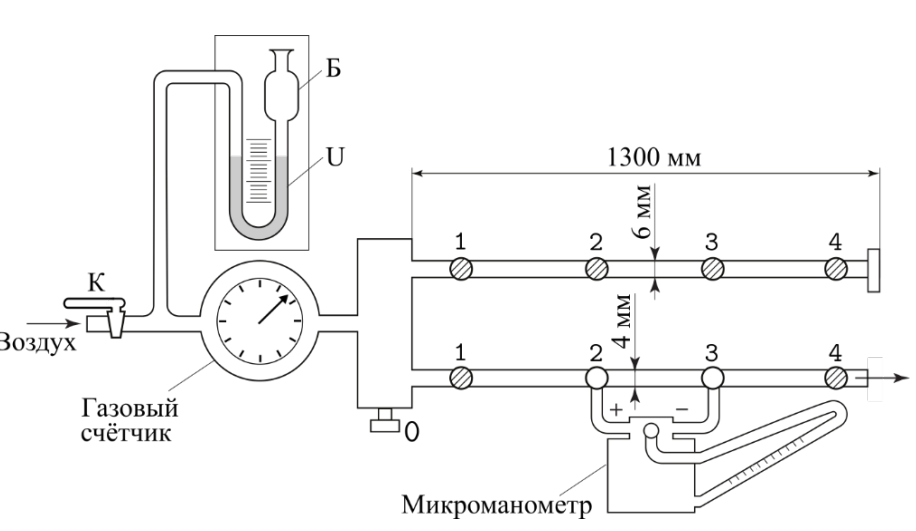
\includegraphics[width=0.5\textwidth]{Установка}
\end{center}
\caption{Схема экспериментальной установки} \label{установка}
\end{figure}
\section{Измерения и обработка данных}
\subsection{Зависимость расхода от перепада давления}
Данные представлены в таблице \ref{Q(P)_tbl} и на графике \ref{Q(P)_pic}.
\begin{table}[h!]
\caption{Зависимость расхода от перепада давления для разных труб}
\label{Q(P)_tbl}
\begin{tabular}{|llll|llll|}
\hline
\multicolumn{4}{|c|}{Ламинарное течение}                                                  & \multicolumn{4}{c|}{Турбулентное течение}                                               \\ \hline
\multicolumn{1}{|l|}{Q, л}   & \multicolumn{1}{l|}{t, с}     & \multicolumn{1}{l|}{N, штрихи}    & d, мм  &\multicolumn{1}{|l|}{Q, л}   & \multicolumn{1}{l|}{t, с}     & \multicolumn{1}{l|}{N, штрихи}    & d, мм   \\ \hline
\multicolumn{1}{|l|}{0.5} & \multicolumn{1}{l|}{86.46} & \multicolumn{1}{l|}{5}    & 3.95 & \multicolumn{1}{l|}{3}   & \multicolumn{1}{l|}{28.77} & \multicolumn{1}{l|}{97}  & 3.95 \\ \hline
\multicolumn{1}{|l|}{1}   & \multicolumn{1}{l|}{65.22} & \multicolumn{1}{l|}{12}   & 3.95 & \multicolumn{1}{l|}{3}   & \multicolumn{1}{l|}{27.58} & \multicolumn{1}{l|}{107} & 3.95 \\ \hline
\multicolumn{1}{|l|}{1}   & \multicolumn{1}{l|}{46.07} & \multicolumn{1}{l|}{17}   & 3.95 & \multicolumn{1}{l|}{3}   & \multicolumn{1}{l|}{26.44} & \multicolumn{1}{l|}{124} & 3.95 \\ \hline
\multicolumn{1}{|l|}{1}   & \multicolumn{1}{l|}{36.32} & \multicolumn{1}{l|}{22}   & 3.95 & \multicolumn{1}{l|}{3}   & \multicolumn{1}{l|}{25.34} & \multicolumn{1}{l|}{144} & 3.95 \\ \hline
\multicolumn{1}{|l|}{1.5} & \multicolumn{1}{l|}{39.05} & \multicolumn{1}{l|}{31}   & 3.95 & \multicolumn{1}{l|}{3}   & \multicolumn{1}{l|}{24.62} & \multicolumn{1}{l|}{162} & 3.95 \\ \hline
\multicolumn{1}{|l|}{1.5} & \multicolumn{1}{l|}{30.64} & \multicolumn{1}{l|}{39}   & 3.95 & \multicolumn{1}{l|}{3.5} & \multicolumn{1}{l|}{27.11} & \multicolumn{1}{l|}{191} & 3.95 \\ \hline
\multicolumn{1}{|l|}{2}   & \multicolumn{1}{l|}{36.67} & \multicolumn{1}{l|}{45}   & 3.95 & \multicolumn{1}{l|}{3.5} & \multicolumn{1}{l|}{25.8}  & \multicolumn{1}{l|}{212} & 3.95 \\ \hline
\multicolumn{1}{|l|}{2}   & \multicolumn{1}{l|}{30.24} & \multicolumn{1}{l|}{55}   & 3.95 & \multicolumn{1}{l|}{3.5} & \multicolumn{1}{l|}{24.22} & \multicolumn{1}{l|}{241} & 3.95 \\ \hline \hline
\multicolumn{1}{|l|}{1}   & \multicolumn{1}{l|}{54.44} & \multicolumn{1}{l|}{4.5}  & 5.1  & \multicolumn{1}{l|}{4}   & \multicolumn{1}{l|}{23.88} & \multicolumn{1}{l|}{64}  & 5.1  \\ \hline
\multicolumn{1}{|l|}{1.5} & \multicolumn{1}{l|}{34.49} & \multicolumn{1}{l|}{11}   & 5.1  & \multicolumn{1}{l|}{5}   & \multicolumn{1}{l|}{28.24} & \multicolumn{1}{l|}{76}  & 5.1  \\ \hline
\multicolumn{1}{|l|}{1.5} & \multicolumn{1}{l|}{24.51} & \multicolumn{1}{l|}{15}   & 5.1  & \multicolumn{1}{l|}{5}   & \multicolumn{1}{l|}{25.45} & \multicolumn{1}{l|}{92}  & 5.1  \\ \hline
\multicolumn{1}{|l|}{2.5} & \multicolumn{1}{l|}{26.8}  & \multicolumn{1}{l|}{23}   & 5.1  & \multicolumn{1}{l|}{5}   & \multicolumn{1}{l|}{20.25} & \multicolumn{1}{l|}{137} & 5.1  \\ \hline
\multicolumn{1}{|l|}{3}   & \multicolumn{1}{l|}{24.77} & \multicolumn{1}{l|}{30}   & 5.1  & \multicolumn{1}{l|}{5}   & \multicolumn{1}{l|}{19.62} & \multicolumn{1}{l|}{148} & 5.1  \\ \hline
\multicolumn{1}{|l|}{2}   & \multicolumn{1}{l|}{27.54} & \multicolumn{1}{l|}{18}   & 5.1  & \multicolumn{1}{l|}{6}   & \multicolumn{1}{l|}{22.48} & \multicolumn{1}{l|}{160} & 5.1  \\ \hline
\multicolumn{1}{|l|}{1}   & \multicolumn{1}{l|}{31.17} & \multicolumn{1}{l|}{8}    & 5.1  & \multicolumn{1}{l|}{}    & \multicolumn{1}{l|}{}      & \multicolumn{1}{l|}{}    &      \\ \hline \hline
\multicolumn{1}{|l|}{0.5} & \multicolumn{1}{l|}{95.33} & \multicolumn{1}{l|}{7}    & 3    & \multicolumn{1}{l|}{2}   & \multicolumn{1}{l|}{22.02} & \multicolumn{1}{l|}{187} & 3    \\ \hline
\multicolumn{1}{|l|}{0.5} & \multicolumn{1}{l|}{40.2}  & \multicolumn{1}{l|}{17}   & 3    & \multicolumn{1}{l|}{2}   & \multicolumn{1}{l|}{23.3}  & \multicolumn{1}{l|}{160} & 3    \\ \hline
\multicolumn{1}{|l|}{0.5} & \multicolumn{1}{l|}{24.69} & \multicolumn{1}{l|}{28}   & 3    & \multicolumn{1}{l|}{2}   & \multicolumn{1}{l|}{25.26} & \multicolumn{1}{l|}{144} & 3    \\ \hline
\multicolumn{1}{|l|}{1}   & \multicolumn{1}{l|}{34.39} & \multicolumn{1}{l|}{40.5} & 3    & \multicolumn{1}{l|}{2.5} & \multicolumn{1}{l|}{25.63} & \multicolumn{1}{l|}{206} & 3    \\ \hline
\multicolumn{1}{|l|}{1.5} & \multicolumn{1}{l|}{42.14} & \multicolumn{1}{l|}{49}   & 3    & \multicolumn{1}{l|}{2.5} & \multicolumn{1}{l|}{25.41} & \multicolumn{1}{l|}{216} & 3    \\ \hline
\multicolumn{1}{|l|}{1.5} & \multicolumn{1}{l|}{32.49} & \multicolumn{1}{l|}{70}   & 3    & \multicolumn{1}{l|}{3}   & \multicolumn{1}{l|}{27.56} & \multicolumn{1}{l|}{258} & 3    \\ \hline
\multicolumn{1}{|l|}{1}   & \multicolumn{1}{l|}{25.41} & \multicolumn{1}{l|}{58.5} & 3    & \multicolumn{1}{l|}{3}   & \multicolumn{1}{l|}{27.38} & \multicolumn{1}{l|}{265} & 3    \\ \hline
\multicolumn{1}{|l|}{1}   & \multicolumn{1}{l|}{38.37} & \multicolumn{1}{l|}{36}   & 3    & \multicolumn{1}{l|}{}    & \multicolumn{1}{l|}{}      & \multicolumn{1}{l|}{}    &      \\ \hline
\end{tabular}
\end{table}
\begin{figure}[h!]
\begin{center}
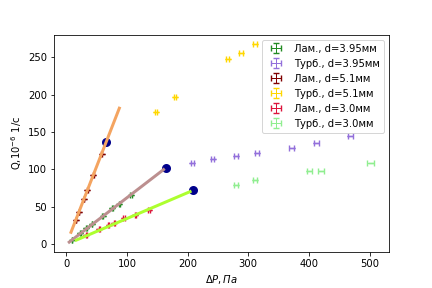
\includegraphics[width=\textwidth]{Q(P)}
\end{center}
\caption{Зависимости расхода
от перепада давления} \label{Q(P)_pic}
\end{figure}

Зависимость $Q(\Delta P)$ представлена на графике, жирными точками обозначены примерные границы перехода от ламинарного течения к турбулентному. Из формулы Пуазейля вычислим коэффициент вязкости воздуха, используя данные ламинарных участках. (табл. \ref{Коэффицент})
\begin{table}[h!]
\caption{Коэффициент вязкости воздуха}
\label{Коэффицент}
\begin{tabular}{|l|l|l|l|}
\hline
d, мм                     & 3.95             & 5.1              & 3.0              \\ \hline
$\eta, 10^-6  Па \cdot c$ & 23.99 $\pm$ 1.24 & 19.97 $\pm$ 0.81 & 14.40 $\pm$ 1.93 \\ \hline
$\epsilon$, \%            & 5.2              & 4.1              & 13.4             \\ \hline
\end{tabular}
\end{table}

Также рассчитаем критическое значение числа Рейнольдса: (табл. \ref{Критическое}). Исходя из полученных значений, критическое число Ренольдса $\sim 10^3$, что согласуется с наблюдениями за столбиком микроманометра.
\begin{table}[h!]
\caption{Критическое число Рейнольдса}
\label{Критическое}
\begin{tabular}{|l|l|l|l|}
\hline
d, мм     & 3.95 & 5.1  & 3.0  \\ \hline
$Re_{кр}$ & 810  & 1020 & 1260 \\ \hline
\end{tabular}
\end{table}

\subsection{Длина установления}
Измерим распределение давление по длине трубки (табл. \ref{распределение})
\begin{table}[h!]
\caption{Распределение давление газа вдоль трубки}
\label{распределение}
\begin{tabular}{|l|l|l|}
\hline
N, штрихи  & x, см     & d, мм    \\ \hline
43 & 130.9 & 3.95 \\ \hline
28 & 80.9  & 3.95 \\ \hline
14 & 40.9  & 3.95 \\ \hline
5  & 10.9  & 3.95 \\ \hline
20 & 30    & 5.1  \\ \hline
39 & 70    & 5.1  \\ \hline
64 & 120   & 5.1  \\ \hline
\end{tabular}
\end{table}
По имеющимся значениям построим график (\ref{P(x)_pic})
\begin{figure}[h!]
\begin{center}
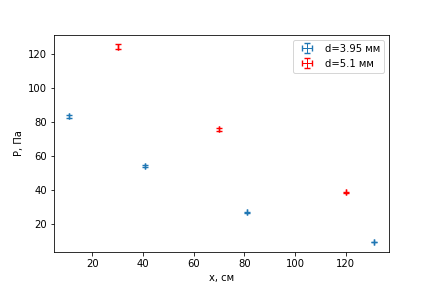
\includegraphics[width=0.95\textwidth]{P(x)}
\end{center}
\caption{Перепад давления от координаты} \label{P(x)_pic}
\end{figure}

Из-за малого числа точек невозможно найти длину установления ламинарного сечения, можно только сказать, что она лежит между 20 и 40 см для $d = 3.95 мм$ и между 40 и 60 см для $d =5.1 мм$, что согласуется с формулой \ref{длина}.

\subsection{Зависимость расхода от радиуса трубки}
Для разных труб при постоянном отношении перепада давления к длине получим \ref{трубы}. Построим график зависимости расхода от радиуса в двойном логарифмическом масштабе \ref{Q(R)}

\begin{table}[h!]
\caption{Измерения на разных трубах}
\label{трубы}
\begin{tabular}{|l|l|l|l|l|l|}
\hline
N, штрихи & l, см & Q, л & t, с  & d, мм & Тип течения  \\ \hline
17        & 0.3   & 0.5  & 41.81 & 3     & Ламинарный   \\ \hline
100.5     & 0.3   & 1.5  & 25.56 & 3     & Турбулентный \\ \hline
17        & 0.3   & 2    & 23.22 & 5.1   & Ламинарный   \\ \hline
134       & 0.4   & 5    & 18.27 & 5.1   & Турбулентный \\ \hline
22.5      & 0.4   & 1    & 30.79 & 3.95  & Ламинарный   \\ \hline
134       & 0.4   & 2.5  & 21.28 & 3.95  & Турбулентный \\ \hline
22.5      & 0.4   & 2    & 18.1  & 5.3   & Ламинарный   \\ \hline
134       & 0.4   & 6    & 23.57 & 5.3   & Турбулентный \\ \hline
22.5      & 0.4   & 3    & 20.8  & 5.85  & Ламинарный   \\ \hline
\end{tabular}
\end{table}

\begin{figure}[h!]
\begin{center}
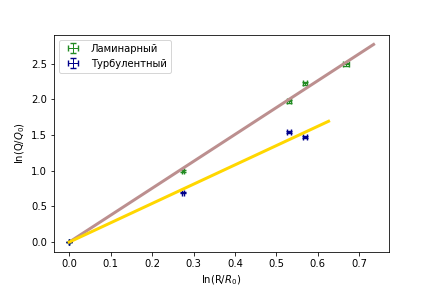
\includegraphics[width=0.95\textwidth]{Q(R)}
\end{center}
\caption{Зависимость расхода от радиуса} \label{Q(R)}
\end{figure}

Наклон для ламинарного $k = 3.70 \pm 0.06$, $k_{теор} = 4$, для турбулентного $k = 2.7 \pm 0.1$, $k_{теор} = 2.5$. Полученные значения достаточно близки к предсказанным теорией.  

\subsection{Зависимость расхода от давления на турбулентном участке}
Используя те же данные (табл. \ref{Q(P)_tbl})  построим график в безразмерных величинах: зависимость числа Рейнольдса от обезразмеренного перепада давления. (\ref{Re(psi)}) При больших числах Рейнольдса (>1700) $\tilde{\psi}$ становится константой, о чем говорит, например, коэффицент наклона прямой через "верхние точки". Так как скоростной напор становится постоянным, то:
\begin{equation}
Q = const \cdot R^{5/2} \sqrt{\frac{\Delta P}{\rho l}}
\end{equation},
что подтверждаеттеоретическую формулу.
\begin{figure}[h!]
\begin{center}
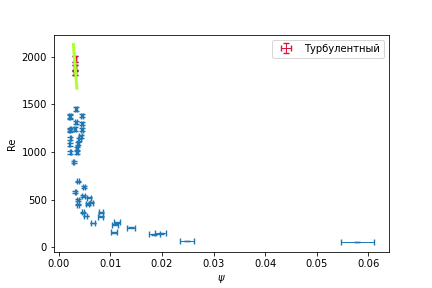
\includegraphics[width=0.95\textwidth]{Re(psi)}
\end{center}
\caption{Зависимость числа Рейнольдса от скоростного напора} \label{Re(psi)}
\end{figure}

\section{Выводы}
\hspace*{20mm}
1. Измерен коэффицент вязкости воздуха: $\eta = 19.45 \pm 1.22 мкПа \cdot c$, теоретическое значение: $\eta = 17.8 мкПа \cdot c$. Значения близки друг к другу.

2. Примерно определена критическая длина трубки, полученное значение согласуется с теоретическим при расчете по формуле: $l_{уст} = 0.2R\cdot Re$

3. Рассмотрена зависимость расхода от радиуса трубки, показатели степени при турбулентном $\beta = 3.70 \pm 0.06$ ($\beta_{теор} = 4$) и ламинарном $\beta = 2.7 \pm 0.1$ ($\beta_{теор} = 2.5$). Экспериментальные значеня не очень существенно отличаются от теоретических.

4. Проанализирована зависимость числа Рейнольдса от скоростного напора, доказана справедливость выражения при турбулентном течении: $Q = const \cdot R^{5/2} \sqrt{\frac{\Delta P}{\rho l}}$ 

\end{document}